\documentclass[portrait,final,a0paper,fontscale=0.277]{baposter}

\usepackage{calc}
\usepackage{graphicx}
\usepackage{amsmath}
\usepackage{amssymb}
\usepackage{relsize}
\usepackage{multirow}
\usepackage{rotating}
\usepackage{bm}
\usepackage{url}

\usepackage{graphicx}
\usepackage{multicol}
\usepackage{palatino}
\usepackage[utf8]{inputenc}
\newcommand{\captionfont}{\footnotesize}

\graphicspath{{images/}{../images/}}
\usetikzlibrary{calc}

\newcommand{\SET}[1]  {\ensuremath{\mathcal{#1}}}
\newcommand{\MAT}[1]  {\ensuremath{\boldsymbol{#1}}}
\newcommand{\VEC}[1]  {\ensuremath{\boldsymbol{#1}}}
\newcommand{\Video}{\SET{V}}
\newcommand{\video}{\VEC{f}}
\newcommand{\track}{x}
\newcommand{\Track}{\SET T}
\newcommand{\LMs}{\SET L}
\newcommand{\lm}{l}
\newcommand{\PosE}{\SET P}
\newcommand{\posE}{\VEC p}
\newcommand{\negE}{\VEC n}
\newcommand{\NegE}{\SET N}
\newcommand{\Occluded}{\SET O}
\newcommand{\occluded}{o}

%%%%%%%%%%%%%%%%%%%%%%%%%%%%%%%%%%%%%%%%%%%%%%%%%%%%%%%%%%%%%%%%%%%%%%%%%%%%%%%%
%%%% Some math symbols used in the text
%%%%%%%%%%%%%%%%%%%%%%%%%%%%%%%%%%%%%%%%%%%%%%%%%%%%%%%%%%%%%%%%%%%%%%%%%%%%%%%%

%%%%%%%%%%%%%%%%%%%%%%%%%%%%%%%%%%%%%%%%%%%%%%%%%%%%%%%%%%%%%%%%%%%%%%%%%%%%%%%%
% Save space in lists. Use this after the opening of the list
%%%%%%%%%%%%%%%%%%%%%%%%%%%%%%%%%%%%%%%%%%%%%%%%%%%%%%%%%%%%%%%%%%%%%%%%%%%%%%%%
\newcommand{\compresslist}{%
\setlength{\itemsep}{1pt}%
\setlength{\parskip}{1pt}%
\setlength{\parsep}{0pt}%
}

%%%%%%%%%%%%%%%%%%%%%%%%%%%%%%%%%%%%%%%%%%%%%%%%%%%%%%%%%%%%%%%%%%%%%%%%%%%%%%
%%% Begin of Document
%%%%%%%%%%%%%%%%%%%%%%%%%%%%%%%%%%%%%%%%%%%%%%%%%%%%%%%%%%%%%%%%%%%%%%%%%%%%%%

\begin{document}

%%%%%%%%%%%%%%%%%%%%%%%%%%%%%%%%%%%%%%%%%%%%%%%%%%%%%%%%%%%%%%%%%%%%%%%%%%%%%%
%%% Here starts the poster
%%%---------------------------------------------------------------------------
%%% Format it to your taste with the options
%%%%%%%%%%%%%%%%%%%%%%%%%%%%%%%%%%%%%%%%%%%%%%%%%%%%%%%%%%%%%%%%%%%%%%%%%%%%%%
% Define some colors
\definecolor{lightgreen}{RGB}{0,205,191}
\definecolor{lightgrey}{cmyk}{0,0,0,0.1}
\hyphenation{resolution occlusions}
%%
\begin{poster}%
  % Poster Options
  {
  % Show grid to help with alignment
  columns=2,
  grid=false,
  % Column spacing
  colspacing=1.25em,
  % Color style
  bgColorOne=lightgrey,
  bgColorTwo=lightgrey,
  borderColor=lightgreen,
  headerColorOne=black,
  headerColorTwo=lightgreen,
  headerFontColor=white,
  boxColorOne=white,
  boxColorTwo=lightgreen,
  % Format of textbox
  textborder=roundedleft,
  % Format of text header
  eyecatcher=true,
  headerborder=closed,
  headerheight=0.1\textheight,
%  textfont=\sc, An example of changing the text font
  headershape=roundedright,
  headershade=shadelr,
  headerfont=\Large\bf\textsc, %Sans Serif
  textfont={\setlength{\parindent}{1.5em}},
  boxshade=plain,
%  background=shade-tb,
  background=plain,
  linewidth=2pt
  }
  % Eye Catcher
  {
  	
\includegraphics[height=6.5em]{ful_logo}
  }
  % Title
  {
  \LARGE
  \textsc{FuL: A Logic processor to aid design and validate virological experiments}\vspace{0.5em}
  }
  % Authors
  {
  	\textsc{Alejandro Kondrasky$^{1}$ - Daniel Gutson$^{1}$ - Carlos Areces$^{2}$}
    \footnotesize{
    \begin{flushleft}
	\hspace{1.5em}$^1$FuDePAN: Fundación para el Desarrollo de la Programación en Ácidos Nucleicos, X5002AOO, Córdoba, Argentina.\\
    \hspace{1.5em}$^2$FaMAF, Universidad Nacional de Córdoba, Ciudad Universitaria, X5000HUA, Córdoba, Argentina.\\
	\end{flushleft}
    }
  }		
  % University logo
  {% The makebox allows the title to flow into the logo, this is a hack because of the L shaped logo.
	\begin{minipage}{12em}
  	
\includegraphics[width=\textwidth]{famaf}\\
  	
\includegraphics[width=\textwidth]{fudepan_logo}
    \end{minipage}
  }

%%%%%%%%%%%%%%%%%%%%%%%%%%%%%%%%%%%%%%%%%%%%%%%%%%%%%%%%%%%%%%%%%%%%%%%%%%%%%%
  \headerbox{Introduction}{name=intro,span=2}{
%%%%%%%%%%%%%%%%%%%%%%%%%%%%%%%%%%%%%%%%%%%%%%%%%%%%%%%%%%%%%%%%%%%%%%%%%%%%%%
	\begin{flushleft}
	\small{
	The body of knowledge in biology, particularly in virology and
	immunology, is increasing in volume and complexity. This is why
	it would be useful to have these knowledge represented in a
	formal language inside a knowledge base. Subsequently, different
	methodologies for analysis and manipulation could be developed,
	allowing validity checks to be performed on conclusions obtained
	in experiments.
	}
	\end{flushleft}
   }
   
   %%%%%%%%%%%%%%%%%%%%%%%%%%%%%%%%%%%%%%%%%%%%%%%%%%%%%%%%%%%%%%%%%%%%%%%%%%%%%%
  \headerbox{Objectives}{name=objective, below=intro}{
%%%%%%%%%%%%%%%%%%%%%%%%%%%%%%%%%%%%%%%%%%%%%%%%%%%%%%%%%%%%%%%%%%%%%%%%%%%%%%
	\small{
	\begin{flushleft}
	FuDePAN's Logic processor (FuL) is being developed to organize, interpret, verify and explore
	knowledge in molecular biology, applied to virology and
	immunology in particular. This will help find inconsistencies and
	automatically derive new information.\\
 	Its main function will be the verification of conclusions obtained by results from
	experiments using queries, as well as assisting in the design of new experiments.
	\end{flushleft}
	}
   }
   
%%%%%%%%%%%%%%%%%%%%%%%%%%%%%%%%%%%%%%%%%%%%%%%%%%%%%%%%%%%%%%%%%%%%%%%%%%%%%%
  \headerbox{Case Study: Junín Virus}{name=problem,below=objective,span=1}{
%%%%%%%%%%%%%%%%%%%%%%%%%%%%%%%%%%%%%%%%%%%%%%%%%%%%%%%%%%%%%%%%%%%%%%%%%%%%%%
	\small{
	\begin{flushleft}
	Our initial test case will be the validation of the
	conclusions obtained by FuDePAN in the Junín experiment about
	the temperature-change effects over the virus secondary
	structure\cite{Junin}:
	\end{flushleft}
	\begin{minipage}{\linewidth}
  	\begin{minipage}{0.5\linewidth}
    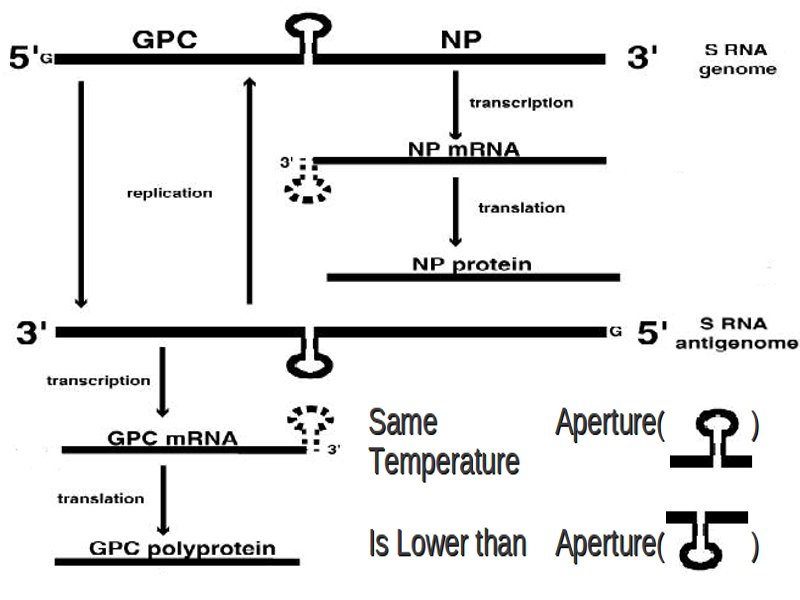
\includegraphics[height=13em]{junin_problem}
  	\end{minipage}\hfill%
  	\begin{minipage}{0.4\linewidth}
    \smaller{
    \vspace{0.5em}
	Corroborate the line of thought that includes the
	predictions of the effects of febrile state over the Junín RNA
	secondary structure: it is hypothesized that the
	temperature increment reduces the production of nucleoproteins
	because the hairpin loop in the intergenic region presents
	dissimilar characteristics when it is compared on the two
	ambisense genome strings when the temperature is increased.
	}
  	\end{minipage}
  	\end{minipage}
	\begin{flushleft}
	A set of definitions and a set of 
	rules was obtained:
	\end{flushleft}
	\resizebox{\linewidth}{!} {
  	\begin{tabular}{l l}
	Definitions								& Rules\\
	\hline
	$S^{+}\equiv$ Genomic RNA produced 
	& 1  $S^{+}\wedge T\implies x(S^{+}\wedge small\_loop)$ \\
	$S^{-}\equiv$ Antigenomic RNA produced 	
	& 2  $S^{-}\wedge T\implies x(S^{-}\wedge\neg small\_loop)$\\
	$NP\equiv$ Nucleoprotein produced 		
	& 3  $S^{+}\wedge small\_loop\implies x(S^{+}\wedge fully\_readable)$\\
	$GPC\equiv$ Glycoprotein produced 		
	& 4  $S^{+}\wedge\neg small\_loop\implies x(S^{+}\wedge\neg fully\_readable)$\\
	$small\_loop\equiv$ Flat intergenic zone 
	& 5  $S^{-}\wedge small\_loop\implies x(S^{-}\wedge fully\_readable)$\\
	$\neg small\_loop\equiv$ Normal intergenic zone 
	& 6  $S^{-}\wedge\neg small\_loop\implies x(S^{-}\wedge\neg fully\_readable)$\\
	$fully\_readable\equiv$ RNA fully readable without cuts 
	& 7  $S^{+}\wedge fully\_readable\implies x(S^{-}\wedge\neg S^{+})$\\
	$\neg fully\_readable\equiv$ RNA not fully readable without cuts 
	& 8  $S^{+}\wedge\neg fully\_readable\implies x(NP\wedge\neg S^{+})$\\
	$T\equiv$ Temperature increase
	& 9  $S^{-}\wedge fully\_readable\implies x(S^{+}\wedge\neg S^{-})$ \\
	$\neg T\equiv$ Temperature decrease 
	& 10 $S^{-}\wedge\neg fully\_readable\implies x(GPC\wedge\neg S^{-})$\\
	& 11 $T\implies x(T)$\\
	& 12 $S^{+}\wedge\neg T\implies x(NP\wedge\neg S^{+})$\\
	& 13 $S^{-}\wedge\neg T\implies x(GPC\wedge\neg S^{-})$\\
	\end{tabular}
    }
    \begin{flushleft}
	Combining this knowledge with the one in a selected knowledge base (KB), 
	the application should be able to validate the conclusions obtained 
	in the Junín experiment\cite{Junin}, using a planner and a semantic 
	reasoner that will process each state of the plan along with the KB and 
	return a new state that will extend it.
	\end{flushleft}
    \begin{center}
	
\includegraphics[width=0.85\linewidth]{1st_approach_1}
	\end{center}
	\begin{flushleft}
	The process will be repeated until a conclusion is reached or a set of questions 
	is obtained for which their answers must be included in the KB in order 
	to advance in the deduction process for answer the original query.
	\end{flushleft}
	}
   }
   
%%%%%%%%%%%%%%%%%%%%%%%%%%%%%%%%%%%%%%%%%%%%%%%%%%%%%%%%%%%%%%%%%%%%%%%%%%%%%%
  \headerbox{Early Design}{name=design,column=1,below=intro}{
%%%%%%%%%%%%%%%%%%%%%%%%%%%%%%%%%%%%%%%%%%%%%%%%%%%%%%%%%%%%%%%%%%%%%%%%%%%%%%
	\small{
	\begin{flushleft}
	FuL has a plug-in architecture, simplifying the inclusion of new kinds of 
	reasoning services. An API will be provided, which defines the way in which 
	knowledge flows between the plug-ins and FuL's core reasoning engine. An SDK 
	composed of libraries and tools required for building plug-ins will also be 
	made available. 
	\begin{center}
	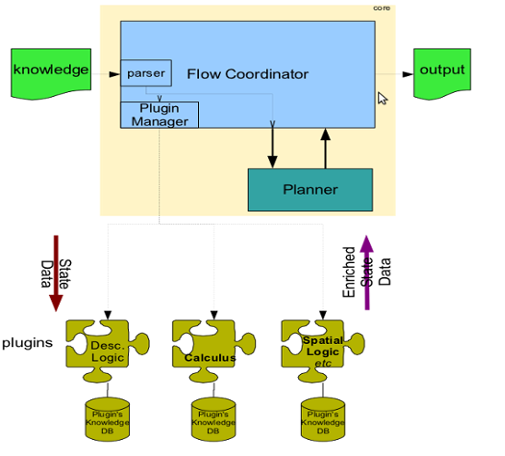
\includegraphics[width=0.9\linewidth]{design}
	\end{center}
	The kernel of the tool will be composed of 
	a planner that can handle PDDL (Planning Domain Definition Language)\cite{PDDL} input, 
	and a KM (knowledge manager) that will be the interface between the plug-ins 
	registered in that session and the planner. During each planner state the deriving 
	process of the next state is as follows :
	\begin{enumerate}
	\smaller{
	\item The KM takes the actual state from the planner and sends it to each registered plug-in.
	\item Each plug-in tries to enrich that state deriving new knowledge by consulting 
		the shared KB and their own.
	\item The knowledge manager generates the derived state by combining the enriched states 
		received from the plug-ins. If there are inconsistencies between the states received from 
		the plug-ins the KM will report this to the user, otherwise it will return the 
		derived state.
	}	
	\end{enumerate}
	FuL will include a semantic reasoner for DL (Description Logics)\cite{DL} as one of the plug-ins.
	We will also provide a knowledge representation language for the virology domain based 
	on DL. 
	This language will allow the development of an ontology of virology knowledge that will be
	available for querying during a FuL session.
	\end{flushleft}
	}
  }
  
%%%%%%%%%%%%%%%%%%%%%%%%%%%%%%%%%%%%%%%%%%%%%%%%%%%%%%%%%%%%%%%%%%%%%%%%%%%%%%
 \headerbox{Features}{name=features,column=1,below=design}{
%%%%%%%%%%%%%%%%%%%%%%%%%%%%%%%%%%%%%%%%%%%%%%%%%%%%%%%%%%%%%%%%%%%%%%%%%%%%%%
	 \begin{flushleft}
	 \small{
	 Via an XML file provided by the user, FuL will register the plug-ins that will 
	 be used during that session and configure different session parameters. 
	 The initial KB file will then be loaded. FuL will process the 
	 KB file with the plug-ins registered in the XML file.
	 Afterwards a prompt-like command line interface will be given to the user with 
	 the following functionalities:
	 \begin{itemize}\itemsep1pt \parskip0pt \parsep0pt
	 \small{
	 \item \textbf{Extend the actual KB with a $\Delta$ KB:} It will 
	 check for inconsistencies and saturate the new KB with atomic concepts derived 
	 from the actual KB $\cup\Delta$KB.
	 \item \textbf{Queries:} The answer of this queries will be consistent with the 
	 actual KB and registered
	 plug-ins. If FuL can not arrive to a conclusion it will return a set of questions 
	 that are unanswerable by FuL. The answers to these questions can be added to the actual 
	 KB in order to return a final answer.
	 }	 
	 \end{itemize}
	 }
	 \end{flushleft}
 }
%%%%%%%%%%%%%%%%%%%%%%%%%%%%%%%%%%%%%%%%%%%%%%%%%%%%%%%%%%%%%%%%%%%%%%%%%%%%%%
  \headerbox{Materials and Methods}{name=method,column=0,below=problem}{
%%%%%%%%%%%%%%%%%%%%%%%%%%%%%%%%%%%%%%%%%%%%%%%%%%%%%%%%%%%%%%%%%%%%%%%%%%%%%%
 \begin{itemize}\itemsep1pt \parskip0pt \parsep0pt
 \footnotesize{
 \item C++: Programming language \url{http://www.open-std.org/jtc1/sc22/wg21/}
 \item FF: Fast Forward Planner \url{http://arxiv.org/abs/1106.0675}
 \item DL: Description Logics \url{http://dl.kr.org/}
 }
 \end{itemize}
 }
%%%%%%%%%%%%%%%%%%%%%%%%%%%%%%%%%%%%%%%%%%%%%%%%%%%%%%%%%%%%%%%%%%%%%%%%%%%%%%
  \headerbox{Repository}{name=source,column=0,below=method,above=bottom}{
%%%%%%%%%%%%%%%%%%%%%%%%%%%%%%%%%%%%%%%%%%%%%%%%%%%%%%%%%%%%%%%%%%%%%%%%%%%%%%
  \footnotesize{
  \noindent
  \begin{minipage}{\linewidth}
  \begin{minipage}{0.85\linewidth}
    \indent{}The repository with the development documentation and, in the near future, source code is available at
  	\url{http://code.google.com/p/ful/}
  \end{minipage}\hfill%
  \begin{minipage}{0.11\linewidth}
  \hfill
\includegraphics[width=\linewidth]{chart}
  \end{minipage}
  \end{minipage}
  }
 }
%%%%%%%%%%%%%%%%%%%%%%%%%%%%%%%%%%%%%%%%%%%%%%%%%%%%%%%%%%%%%%%%%%%%%%%%%%%%%%
  \headerbox{References}{name=references,column=1,below=features,above=bottom}{
%%%%%%%%%%%%%%%%%%%%%%%%%%%%%%%%%%%%%%%%%%%%%%%%%%%%%%%%%%%%%%%%%%%%%%%%%%%%%%
    \scriptsize{
    \bibliographystyle{ieee}
    \renewcommand{\section}[2]{\vskip 0.05em}
      \begin{thebibliography}{1}\itemsep=-0.5em
      \setlength{\baselineskip}{0.5em}
      \bibitem{DL}
        \begin{minipage}{\linewidth}
        Franz Baader, Deborah L. McGuinness, Daniele Nardi, Peter F. Patel-Schneider.
  		\end{minipage}
        \begin{minipage}{\linewidth}
        The Description Logic Handbook: Theory, implementation, and applications.
  		\end{minipage}
      \bibitem{PDDL}
        \begin{minipage}{\linewidth}
        The Seventh International Planning Competition Description of
		Participant Planners of the Deterministic Track.	
 		In {\em 2011}
  		\end{minipage}
		\begin{minipage}{\linewidth}
		\begin{minipage}{0.85\linewidth}
		\bibitem{Junin}
      	  Daniel Gutson, Agustín March, Maximiliano Combina, Daniel Rabinovich.\\	
		  Prediction of consequences of the febrile status on the RNA secondary structure of the Junín Virus
          In {\em 2006} \url{http://www.fudepan.org.ar/node/71}
         \end{minipage}
		 \begin{minipage}{0.14\linewidth}
		  \begin{center}
		  \hfill
\includegraphics[width=0.85\linewidth]{junin_qrcode}
		  \end{center}
		 \end{minipage}
		\end{minipage}
      \end{thebibliography}
    }
  }

\end{poster}

\end{document}

